\chapter{Estudo de Caso}
\label{cap:estudo-de-caso}

Nesse estudo de caso, nos buscamos atingir três objetivos: (1) garantir a
replicabilidade dos resultados, (2) construir uma estrutura que possa ser
estendida para outros cenários e (3) validar os problemas associados com novas
abstrações de processos. Temos uma estrutura para implantação (\emph{deploy})
que é responsável por configurar todas as máquinas alvos envolvidas nos
experimentos, para automatizar tal passo, decidimos utilizar a ferramenta
\emph{Ansible} para controlar o \emph{deploy} uma vez que esta é amplamente
utilizada e é relativamente simples de se utilizar. Adicionalmente, temos um
grupo de scripts projetados para estressar diferentes cenários, esses scripts
são baseados em uma ferramenta chamada \emph{Apache Benchmark Tool} (ab) que
por sua vez tem configurações específicas para estressar diferentes aspectos do
SO e do servidor de HTTP. Temos uma coleção de programas para processar todos
os dados gerados durante a execução do experimento e produzir os gráficos.
Nesse capitulo, nos detalhamos nosso experimento e como no desejamos verificar
os benefícios da abordagem utilizando Múltiplos Endereços Virtuais (MVAS).

\section{Metodologia}
\label{sec:metodologia}

\begin{figure}[!h]
  \centering
  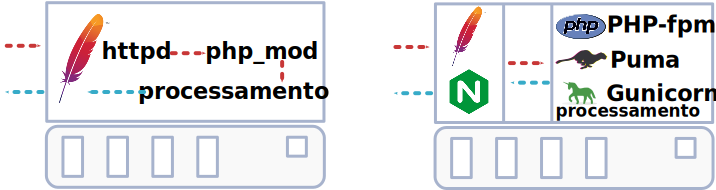
\includegraphics[width=.60\textwidth]{web_server_organization_strategy}
  \caption{Web server organization}
  \label{fig:web_server}
\end{figure}

Atualmente podemos encontrar um grande número de arquiteturas que podem ser
utilizadas por um sistema web. A Figura \ref{fig:web_server} ilustra duas
arquiteturas diferentes. A primeira mostra uma situação na qual uma página web
é totalmente manipulada pelo Apache HTTPD. Basicamente, o HTTPD manipula uma
solicitação e passa ela para um módulo específico responsável por executar um
software (e.g.: uma página web em PHP é executado por um módulo PHP). A segunda
arquitetura é um exemplo de página web escrita em \emph{Ruby on Rails} que é
composta de duas camadas: (1) um servidor web para manipular as requisições que
chegaram dos clientes (pode ser o Apache ou Nginx), (2) um servidor de
aplicação responsável por executar um programa (no exemplo da figura, temos o
PUMA que é especializado em executar código Ruby). Esses exemplos, ilustram que
no podemos ter diferentes formas de organizar a arquitetura.

\begin{figure}[!h]
  \centering
  \includegraphics[width=.90\textwidth]{experiment_arhitecture}
  \caption{Arquitetura do experimento}
  \label{fig:experiment_architecture}
\end{figure}

A Figura  \ref{fig:experiment_architecture}, ilustra de forma geral a estrutura
utilizada para conduzir os experimentos com MVAS. Note que a figura indica duas
máquinas virtuais (Host 1 e Host 2), uma com um servidor web configurado para
dar suporte para um grande número de requisições geradas por uma segunda
máquina, que por sua vez, é responsável por simular um grande número de
clientes concorrentes. Ambas as máquinas são conectadas via conexão Gigabit
Ethernet, uma vez que queremos simular múltiplos cliente fazendo requisições
sem ter que se preocupar com questões de sobrecarga da rede.

Nos experimentos, nos queremos simular uma situação na qual o HTTPD terá que
lidar com uma enorme carga que gere grande pressão na aplicação e assim
elevando a utilização de recursos de hardware. Com essa ideia em mente, nos
conduzimos dois experimentos empíricos com o objetivo de determinar qual seria
a configuração ideal para o Host 1. Primeiro, nos investigamos as principais
características das diferentes estrategias de MPM e notamos que o
\emph{Prefork} tem um grande consumo de memória; por isso, a quantidade de
memória foi escolhida com base no \emph{Prefork} uma vez que se espera que as
estratégias de \emph{Worker} e \emph{Event} consumam menos memória. Em segundo
lugar, nos conduzimos um pequeno conjunto de experimentos com diferentes cargas
de trabalho (\emph{workload}) e monitoramos a utilização de recursos. Nos
analisamos os logs e concluímos que a forma mais rápida de tornar evidente a
diferença entre as estratégias é a de utilizar poucos núcleos e ter um bom
tamanho de memória. Consequentemente, nos decidimos utilizar uma máquina de
13GB de memória RAM e 2 núcleos. Note que 13GB é um tamanho selecionado visando
dar suporte para um grande número de requisições quando o HTTPD é configurado
para utilizar o \emph{Prefork}. Finalmente, é importante ressaltar que o Host 1
tem uma ferramenta configurada para monitorar a utilização de memória e CPU
(Collectl\footnote{http://collectl.sourceforge.net/ Accessed at 2017/07/03})
que é posteriormente recuperada para analise.

A segunda máquina, tem uma coleção de scripts que utiliza a ferramenta de
Benchmark do Apache (ab) para gerar diferentes testes; a Figura
\ref{fig:experiment_architecture} ilustra a máquina que é responsável por
produzir diferentes cargas. Todas as requisições são monitoradas e salvas em
arquivos. Depois, todas as informações produzidas pela segunda máquina são
recuperadas e processadas.

\section{Customizações no servidor Apache e no GNU/Linux}
\label{sec:customization}

Uma das principais características do HTTPD é a sua habilidade de ser
facilmente ajustado por meio de arquivos de configuração. Da perspectiva de um
usuário avançado, o Apache HTTP pode ser mais flexível e adaptável para
diferentes contextos. Apesar de toda a flexibilidade e capacidade do HTTPD,
esse vem com uma configuração conservadora por padrão para evitar que os
usuários não experientes causem algum tipo de dano ao seu próprio ambiente.
Consequentemente, é necessário configurar o HTTPD para suportar grandes cargas
de requisições. Da mesma forma, o GNU/Linux também vem configurado de maneira
conservadora e esse também possibilita um elevado grau de personalização.
Portanto, um usuário avançado que desejar fazer com que o Linux entregue o
melhor desempenho possível para cada hardware, o mesmo deve personalizar vários
arquivos internos (em alguns caso, até recompilar o Kernel). Nesse trabalho,
nos queremos simular uma situação que se assemelhe a de um servidor web que
manipule uma elevada carga de requisições, por isso, nesse trabalho fizemos
diversas otimizações no servidor Apache e no Linux.

Nos nossos experimentos, nos utilizamos e comparamos: \emph{Prefork},
\emph{Worker} e \emph{Event}. Todas as estratégias de MPM tem um arquivo de
configuração especifico associado, na qual cada um permite algum tipo de ajuste
fino. Seguem os principais parâmetros disponíveis para configurar esse tipo de
MPM 

\begin{itemize}
  \item \textbf{StartServers}: This parameter expects a positive integer, which
        will represent the total of processes that will start at the HTTPD
        initialization. The default value is different between the MPMs
        \cite{mpm_start_server};
  \item \textbf{MinSpareServers}: This parameter expects a positive integer,
        and setting up the minimum number of idle process. It is important to
        have a pool of idle processes, because in the case that HTTPD receives
        a large amount of request in a short time interval, the idle children
        may be used for trying to attend all the request. The parent process
        compares the total amount of idle children with the
        \textit{MinSpareServers} number. If it has fewer idle children than
        MinSpareServers, the parent process creates new
        children \cite{mpm_min_spare};
  \item \textbf{MaxSpareServers}: This parameter expects a positive integer,
        and setting up the maximum number of idle process. Note that
        \textit{MinSpareServers} and \textit{MaxSpareServers} work together,
        controlling the total of resources being used by children
        processes \cite{mpm_max_spare};
  \item \textbf{MaxRequestWorkers}: This parameter sets the total number of
        requests served by the HTTPD. If the number of requests is higher than
        \textit{MaxRequestWorkers}, then all new requests will be queued. The
        size of the Apache HTTPD queue is configured in \textit{ListenBacklog}
        parameter \cite{mpm_max_request};
  \item \textbf{ListenBacklog}: It is the maximum length of the waiting queue.
        This value has a relation with the TCP queue size defined in the
        GNU/Linux \cite{mpm_listen};
  \item \textbf{ServerLimit}: Increase the total number of processes allowed
        by the HTTPD \cite{mpm_server_limit}.
  \item \textbf{MinSpareThreads}: This parameter expects a positive integer,
        which represents the minimum number of idle threads. If there are many
        requests to the server, and there are not enough idle threads to handle
        the load, the child process creates more threads until it achieves a
        greater number than the one set in this parameter. By default, the
        HTTPD set a value of 75 to this parameter \cite{mpm_minsparethreads}.
  \item \textbf{MaxSpareThreads}: This parameter expects a positive integer,
        which represents the maximum number of idle threads. If the HTTPD has
        more idle threads than the number specified in this parameter, the
        child process is killed. By default, this value is set to 100
        \cite{mpm_maxsparethreads}.
  \item \textbf{ThreadLimit}: This parameter expects a positive integer, which
        represents the upper limit of threads per process
        \cite{mpm_threadlimits}.
  \item \textbf{ThreadPerChild}: This parameter expects a positive integer,
        which represents the total of threads per child process
        \cite{mpm_threadperchild}.
\end{itemize}

\begin{table}
  \centering
  \begin{tabular}{|c|c|c|c|}
    \hline
    \textit{Parameter} & \textbf{Event} & \textbf{Worker} & \textbf{Prefork} \\
    \hline
    \textbf{ServerLimit} & 6000 & 6000 & 5000\\
    \hline
    \textbf{StartServer} & 10 & 10 & 1000\\
    \hline
    \textbf{MinSpareThreads} & 512 & 512 & --\\
    \hline
    \textbf{MaxSpareThreads} & 1024 & 1024 & --\\
    \hline
    \textbf{ThreadLimit} & 64 & 64 & --\\
    \hline
    \textbf{ThreadPerChild} & 64 & 64 & --\\
    \hline
    \textbf{MaxRequestWorkers} & 5120 & 5120 & 5000\\
    \hline
    \textbf{MinSpareServers} & -- & -- & 500\\
    \hline
    \textbf{MaxSpareServers} & -- & -- & 1500\\
    \hline
  \end{tabular}
  \caption{MPM configurations}
  \label{tab:configuration}
\end{table}

Table \ref{tab:configuration}, illustrates our HTTPD customization. Our setting up allowed Apache
HTTPD to reply a large number of requests which made the experiments closer to
a real situation. Our customizations in GNU/Linux and in the HTTPD, enabled us
to make Apache HTTPD using all the available hardware resources.

\begin{table}
  \centering
  \begin{tabular}{|c|c|}
    \hline
    \textit{parameter} & \textbf{value}\\
    \hline
    Max queue events & 1048576\\
    \hline
    Max user instances & 1048576\\
    \hline
    Max user watches & 1048576\\
    \hline
    Max map count & 262144\\
    \hline
    TCP max syn backlog & 8096\\
    \hline
    TCP syncookies & 0\\
    \hline
  \end{tabular}
  \caption{Kernel configurations}
  \label{tab:kernel_config}
\end{table}

Secondly, it is required to customize the GNU/Linux since it has a default
behavior to avoid any application to consume the entire hardware resources
(e.g.; the HTTPD). Table \ref{tab:kernel_config}, compiles all the GNU/Linux
customization adopted by us. First, the GNU/Linux establishes a limit of open
File Descriptor (FD), which is a problem in our case because the HTTPD handles
a large number of requests and each request holds one FD. To overcome this
problem, we increased the total amount of the file descriptor (Table
\ref{tab:kernel_config}, Max map count parameter) supported by the Kernel to a
large number, which allows the HTTPD to handle more requests. Second, the
GNU/Linux has a collection of configurations files that prevents some
well-known network attack. In our case, we disabled the SYN Flood protection
(Table \ref{tab:kernel_config}, TCP syncookies), since this feature blocks the
massive number of requests made by us. Third, the default wait queue of the TCP
layer is small for our case, therefore, we increase this value to a large
number (Table \ref{tab:kernel_config}, TCP max syn backlog, Max queue events,
and Max user instances).

In conclusion, we ostensibly tune the HTTPD and GNU/Linux to accept a large
number of requests. These configurations are important to our context once we
wish to put the HTTPD under pressure to show us MVAS behavior in this
situation.

\section{Scenarios}

It is common to find application running on the HTTPD that demands to work with
a database. Usually, this sort of application has to wait for the database
operation returns any data. This scenario can be easily expanded to a situation
with a large amount of request or with a busy database. Sometimes, Server-side
applications also have cache strategies, which generates a completely new
scenario. With this idea in mind, we had to decide on what kind of experiment
we want to conduct. This section described our current scenario. 

\subsection{Selected Scenarios}
\label{sec:scenarios}

\begin{table}[!h]
  \centering
  \begin{tabular}{|c|c|c|}
    \hline
    & \textbf{Small} & \textbf{Large}\\
    \hline
    Static & 70Kb & 120Kb\\
    \hline
    Dynamic & 80Kb & 120Kb \\
    \hline
  \end{tabular}
  \caption{File size to transfer}
  \label{tab:file_size}
\end{table}

Our experiment was composed of four different scenarios, separated by two file
types: static and dynamic. First, we employed two distinct static files (pure
HTML), and each one differentiates only by their size. Table
\ref{tab:file_size} shows both file sizes adopted for the static file, and
those values are based on the HTTP Achieve report of 2015 wherein the average
size of an HTML file is 66KB \cite{httparchive}.  Second, for the dynamic
files, it was written a simple Python code that generates a different output
per request. We decided by this strategy with dynamic files as a way to avoid
the system cache.  Finally, the dynamic file is important in this scenario as a
way to keep the CPU utilization for a long time and the file size can affect on
it.

The HTTPD delivers static HTML documents with a low hardware utilization
because these files do not require a large data processing. These
characteristics are desirable to show the difference between Prefork, Event,
Worker, and MVAS inside Apache Server with a small influence of the CPU. On the
other hand, the dynamic files used in this experiment are CPU bound and aimed
to simulate a situation wherein requests have to wait for data processing. This
situation overloads the CPU and as a consequence, it consumes a large amount of
memory since threads or processes have to live until the end of the processing.

\begin{table}[h!]
  \centering
  \begin{tabular}{|c|c|c|}
    \hline
    Cases & \textbf{Requests} & \textbf{Concurrency}\\
    \hline
    Static files & 60000 & 20000\\
    \hline
    Dynamic files & 5000 & 600 \\
    \hline
  \end{tabular}
  \caption{Main loads applied}
  \label{tab:loads}
\end{table}

Table \ref{tab:loads} illustrates the load applied in the experiments. For
static files, we applied a large number of requests with a high level of
concurrency. For dynamic files, we applied a lower number of requests with a
small level of concurrency. Our goal with this configuration is examining if it
is possible to answer the research question 1 and 2. For this task, we are not
using the keep-alive feature.

\section{MVAS inside GNU/Linux and Apache HTTP Server}
\label{sec:mvas_inside_httpd}

\subsection{MVAS inside GNU/Linux}
 
SpaceJMP \cite{spacejmp} was the first implement of MVAS concepts, and it is
available for DragonFlyBSD and Barrelfish. In 2016 the researchers decided to
implement MVAS on Linux kernel with the intention to extend the original work
and send the modification as a patch to the Linux project. As a result, in
August 2016, was released the first version of MVAS for Linux
\footnote{https://github.com/l3nkz/linux/tree/mvas Accessed at 2017/07/03}.
 
For using the current MVAS implementation on Linux, we work in a repository
forked from the original Kernel by Till Smejkal (the original author of MVAS in
Linux). During our tasks, we had to learn how to compile, customize, and
install our own version of the Linux Kernel. To support this activity, we
installed Debian OS and changed the Kernel for our custom version. We already
understand all the processes and every new release of MVAS we just update our
Kernel.
 
MVAS is accessible through system call, and also has some debug information
which helps to track problems. Additionally, we study the current
implementation of MVAS for better understand it and sometimes we provide
feedback for the developer. Currently, Till Smejkal is not working on the
patch, but another employee from HPe (Ranjan Sarpangala) maintain the MVAS
evolution.

\subsection{MVAS inside Apache HTTP Server}

A request has a short lifecycle inside the HTTPD, since it is created and
destroyed frequently. The information about a client and its connection are
stored inside the request data structure. From the security perspective, it is
desirable to totally isolate each request. Also, the isolation should not
impose a high performance penalty, otherwise it cannot be used inside HTTPD.
Although the Process-based directly isolates all the requests, it generates a
large memory footprint (Section \ref{sec:prefork}). On the other hand, the
Thread-based strategy has a better performance but it is not fully isolated.

MVAS has a mechanism for creating multiple virtual address spaces, all entirely
isolated and with a persistent behavior (Section \ref{sec:mvas}). We believe,
that the aforementioned properties allow the implementation of a hybrid system
with the same level of isolation provided by processes and with similar threads
performance. We appended MVAS on the request lifecycle. Our intention is
checking if it can add an extra level of isolation to request, while keeping a
similar performance of threads.

\begin{figure}[!h]
  \centering
  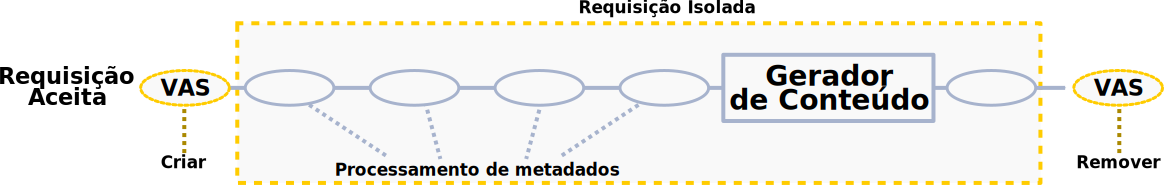
\includegraphics[width=.99\textwidth]{mvas_httpd} 
  \caption{HTTPD with MVAS}
  \label{fig:httpd_mvas} 
\end{figure}

Figure \ref{fig:httpd_mvas}, shows our approach for adding MVAS inside the
HTTPD. Before the request data structure be built in Apache HTTP server, we
create a new VAS, attach it to the current thread, and switch to the new VAS.
Afterward, all the request life cycle will be performed as usual, but inside
the new VAS (totally isolated). When the request finishes, we proceed with the
clean up the information related to the VAS. This approach, guarantees the
total isolation of any new request.

The aforementioned approach gives a theoretical idea of how we added the
isolation provided by MVAS inside the Apache HTTP Server. We had to look
closely to the HTTPD code to find the correct place to add a full isolation
into the request in a thread-based strategy. Our first attempt was trying to
extend the Worker model and adapted it to use MVAS. However, after weeks of
work in this new MPM model, we realized that is a large effort for something
that may not work as we expected. We decided to discard this approach for a
while and find another way to add the MVAS isolation.
 
Our second approach is simpler than the idea of creating a new MPM module, and
with the advantage of request isolation. We identified the exact functions that
keep the entire request lifecycle, from the beginning to the end, and applied
the MVAS isolation. These functions name are:
\texttt{process\_http\_async\_connection} and
\texttt{ap\_process\_http\_sync\_connection} (both located in the file
\texttt{modules/http/http\_core.c}). MPM modules invoke one of this functions
for handling the request lifecycle, for this reason, adding MVAS on these
functions eliminate the complexity related to the code. However, this
alternative adds isolation for all the request which can generate unnecessary
overhead. 

Code \ref{lst:http_core} is a snippet of code extracted from our implementation
of MVAS inside the Apache HTTP Server. Notice that
\texttt{create\_isolate\_vas} function is designed to support the creation of
new VAS inside the Apache HTTP. Code \ref{lst:http_core} also shows
\texttt{ap\_process\_http\_async\_connection} and
\texttt{ap\_process\_http\_sync\_connection} functions and both are isolated
inside a new VAS. At the beginning of each of these functions, it is created a
new VAS, attached it to the current process, and finally switched to the new
VAS before the HTTPD create the request. In the end of request lifecycle, we
deleted the VAS. Our current implementation still needs improvements, but it is
already functional. Finally, all the source code of our modification is
available on GitHub at
\url{https://github.com/LSS-USP/httpd-experiment/tree/mvas\_worker}.

\lstinputlisting[
                 language=C,
                 caption={Simple example of threads in action},
                 label={lst:http_core}
                ]{code/http_core.c}

We expected that MVAS adds some extra latency, however, we want to investigate
if the additional overhead is tolerable or not. With this experiment with
HTTPD, we want to see if threads with MVAS can replace the use of processes in
some situations.

\section{Preliminary Results}
\label{sec:preliminary}

The method proposed in Section \ref{sec:metodologia} emerged from
our work to answer the first research question. In this sense, we already
implemented and tested our approach and get some results for the first
question. Currently, we are working on the second question. This section will
present our preliminary results and discussions about them.

\subsection{Q1: Is There a Significant Performance Difference Between the Apache HTTP Server Working With Processes and Apache HTTP Server Working With Threads?}
 
In the first scenario, we have the HTTPD with the customizations explained in
Section \ref{sec:customization} but without the MVAS modification. Answering
this question provides three advantages: (1) point the differences between
process- and thread-based strategies, (2) the HTTPD behavior without MVAS for
later comparison, and (3) validate the methodology.
 
\begin{table}[h!]
  \centering
  \begin{tabular}{|c|c|c|}
    \hline
    Name & \textbf{Cores} & \textbf{Memory}\\
    \hline
    M1 & 2 & 13Gb \\
    \hline
    M2 & 2 & 4Gb \\
    \hline
  \end{tabular}
  \caption{Hardware}
  \label{tab:machines}
\end{table}

In the Section \ref{sec:metodologia} and Section
\ref{sec:scenarios}, it is detailed our methodology and the basic setup wherein
we strictly followed. Two hardware platforms support our measurements,
code-named M1, and M2, as shown in Table \ref{tab:machines}. Note that we
decided to use a few cores and a large memory since these conditions can better
reveal the limitation related to the HTTPD.
 
\begin{figure}[!h]
  \centering
  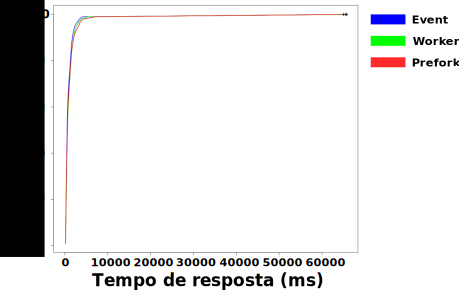
\includegraphics[width=.90\textwidth]{static_file}
  \caption{Static file: Time taken to serve the percentage of request}
  \label{fig:static_file}
\end{figure}

The graph in the Figure \ref{fig:static_file} shows a percentage in the y-axis,
and the x-axis has the time it took to serve that the percentage of request
\cite{apache_ab}. Note that Figure \ref{fig:static_file} illustrates the
scenario with static files wherein the web server has to handle 60000 requests,
simulating 20000 requests in parallel. Furthermore, the graphics illustrate
prefork, work, and event together to better show the differences between them.

\begin{figure}[!h]
  \centering
  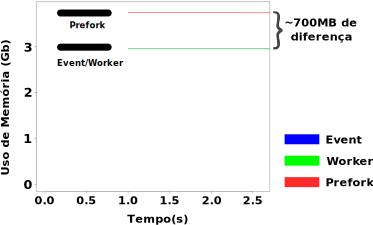
\includegraphics[width=.90\textwidth]{static_file_memory_usage}
  \caption{Static file: Memory consumption required to serve all the requests}
  \label{fig:static_file_memory}
\end{figure}
 
Analyzing the Figure \ref{fig:static_file}, it is possible to note that the
response time was almost the same for all the MPM strategies. On a first
analysis,  this results can seem frustrated since the prefork is based on
processes. Nevertheless, Figure \ref{fig:static_file_memory} presents the
experiment from the memory perspective. Note that prefork uses around 3.7Gb and
event/worker require 3Gb for handling all the requests. This results clearly
show the disadvantage of using a prefork even for a simple case. Lastly, it is
important to highlight that threads and processes had the same response time in
this case since the overhead for processes and thread switching are the same in
the GNU/Linux \cite{linux_kernel_development}.

\begin{figure}[!h]
  \centering
  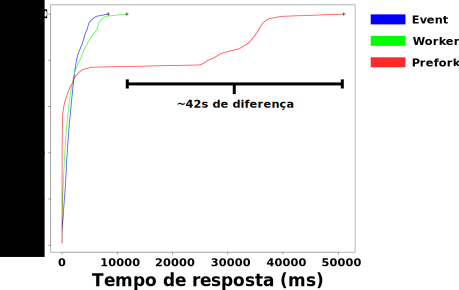
\includegraphics[width=.90\textwidth]{dynamic_file_request_time}
  \caption{Dynamic file: Time taken to serve the percentage of request}
  \label{fig:dynamic_file}
\end{figure}

\begin{figure}[!h]
  \centering
  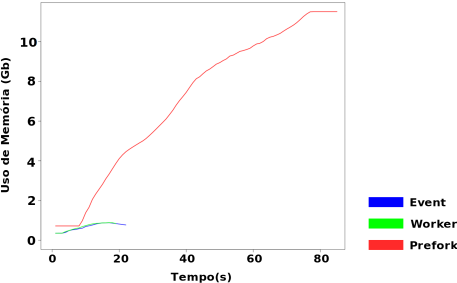
\includegraphics[width=.90\textwidth]{dynamic_file_memory_usage}
  \caption{Dynamic file: Memory consumption required to serve all the requests}
  \label{fig:dynamic_file_memory}
\end{figure}

Figure \ref{fig:dynamic_file} shows a scenario with the dynamic file. In this
case, the difference between process and threads are much more clear. Prefork
is much slower than Event and Worker, the difference is close to 42 seconds
which is unacceptable in a real situation. To better understand the situation,
Figure \ref{fig:dynamic_file_memory} illustrates the memory usage and it is
explicit that Prefork has a huge memory footprint when it is compared with
Event and Worker. This situation can be examined from the OS perspective, the
HTTPD has to create one child process per request and keep them alive until it
finishes all the request processing. As a result, the HTTPD has numerous
processes alive and consuming memory. On the other hand, threads share data
with the parent process which reduces the memory footprint, hence, keeping
threads alive during the request is cheaper.

In conclusion, it is clear there is an enormous difference between processes
and threads inside the HTTPD. By partially answering this question, we find two
distinct scenarios and load that can show the MPM differences. The current
results, provide the basic information required by the rest of this work. We
expected to improve our scenarios and load for the next iterations of this
work.
 
\subsection{Q2: What is the Performance Difference Between the Apache HTTP Server Running With MVAS, With a Process-based Strategy, and With a Thread-based Strategy?}

Based on the results from the first research question, we started to work to
add MVAS inside the HTTPD. As explained in Session \ref{sec:mvas_inside_httpd},
we already have a modified version of the HTTPD code using MVAS. We installed
our HTTPD version and executed the benchmark again. However, our experiments
with MVAS pointed three problems: (1) it does not work with multiple threads,
(2) it has allocation problems, and (3) there is a large overhead in MVAS
operations.

For the first problem, we had conversations with the MVAS authors for trying to
identify the issue. After inspections in the implementation, authors detected
some problems on their heuristics for handling memory segments. Basically, MVAS
has problems related to the stack allocation. Unfortunately, solving this
problem will require change many parts of the current implementation.
 
\begin{figure}[!h]
  \centering
  \includegraphics[width=.70\textwidth]{mvas_problem}
  \caption{Linux memory allocation with malloc, image based on \cite{kernel_malloc}}
  \label{fig:malloc_linux}
\end{figure}
 
For the second problem, we first have to understand how Linux allocate memory.
Figure \ref{fig:malloc_linux} illustrates the heap segment for a program and in
the physical memory. Notice from the first part of the Figure
\ref{fig:malloc_linux} that heap is mapped to physical memory. Next, the
program asks for more memory to the OS via malloc function. Linux just extends
the heap segment size, and return a new reference to the program. Note that
Linux does not map heap into the physical memory directly, it waits for the
program try to write something in the memory. Just after an attempt to write in
the memory the Kernel really allocates the physical memory for the program.
With this idea in mind, MVAS have to handle this situation and here is the
problem. Unfortunately, MVAS fail to map this situation and each VAS switch
lost the reference to the physical memory.
 
For the third problem, we try to figure out what is the real problem.
Currently, we try to find the bottleneck by measuring the VAS operations
(create, attach, switch, detach, and delete) inside the HTTPD, but we did not
identify the problem yet.
